\documentclass[tikz, margin=2mm,convert={density=300,size=1920x1080,outext=.png}]{standalone}

\usepackage{xcolor}
\usetikzlibrary{decorations.pathreplacing}

\newcommand{\len}{5}
\newcommand{\bre}{1}

\begin{document}
    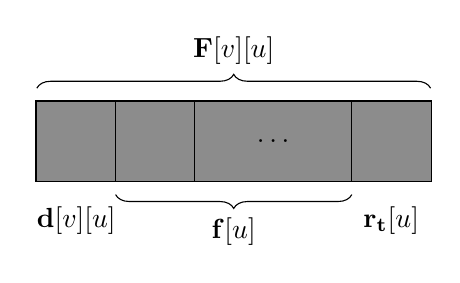
\begin{tikzpicture}[>=stealth]
        \coordinate (O) at (0, 0);
        \coordinate (A) at (\len, 0);
        \coordinate (B) at (0, \bre);
        \coordinate (C) at (\len, \bre);
        \draw[line width=1.25pt] (O) -- (A) -- (C) -- (B) -- cycle;
        \fill[black!45!white] (O) -- (A) -- (C) -- (B) -- cycle;
        % dotted lines
        \foreach \x in {1, ..., 4} {
            \ifnum\x=3
                \node[draw=none]  at (\x, .5) {$\ldots$};
            \else
                \draw[-] (\x, 0) -- (\x, 1);
            \fi
        }
        % labels
        \draw[decoration={brace,raise=5pt, amplitude=5pt},decorate] (0,1) -- node[above=10pt] {$\mathbf{F}[v][u]$} (5,1);
        \node[draw=none] at (.5, -.5) {$\mathbf{d}[v][u]$};
        \draw[decoration={brace,mirror,raise=5pt, amplitude=5pt},decorate] (1,0) -- node[below=10pt] {$\mathbf{f}[u]$} (4,0);
        \node[draw=none] at (4.5, -.5) {$\mathbf{r_t}[u]$};
        
    \end{tikzpicture}
\end{document}